%Preamble
\documentclass[11pt]{article}
%packages
\usepackage[margin=1in]{geometry}
\usepackage{tabularx}
\usepackage{multirow}
\usepackage{array}
\usepackage{fancyhdr}
\usepackage{amsmath,amssymb,amsthm}
\usepackage{float}
\usepackage{graphicx}
\graphicspath{{../images/}}
\usepackage[section]{placeins} %for FloatBarrier
\usepackage[hidelinks]{hyperref}
\usepackage{xcolor,soul}
\definecolor{linkcolor}{HTML}{0066ff}
\newcommand{\link}[2]{\href{#1}{\color{linkcolor}\setulcolor{linkcolor}\ul{\mbox{#2}}}}
%Refernces
\usepackage[natbib=true,
            bibencoding=utf8,
            style=authoryear,
            backend=biber,
            %autocite=superscript,
            sorting=none,
            useprefix=true]{biblatex}
\addbibresource{../refs.bib}


\begin{document}

\title{{\Huge02-601: Final Project Essay}\\
        SELEXzyme: Generating DNAzymes \\
        with a Genetic Algorithm}
\author{Siddharth Reed, slreed}
\date{December 11, 2020}
\maketitle
\section*{Background}
\paragraph{\textbf{DNAzymes}}
A DNAzyme is a single-stranded DNA sequence that has some king of catalytic activity \citep{dnazyme}.
These sequences are generally short ($< 100$bp) and rely on some kind of tertiary structure for their catalytic activity.
Such sequences have never been observed in nature but have been developed synthetically by researchers \citep{selex}.
Using a method known as SELEX researchers are able to start with a large random pool of sequences and evolve them for a specific purpose \citep{selex}.
In the case of DNAzymes that purpose is to catalyze some specific reaction, often the cleavage of some target RNA sequence.
So a pool of sequences is incubated with the cleavage target and there is a selection method to isolate only those sequences that cleaved the target.
These sequences are isolated and amplified in such a way as to introduce some variation into the sequences.
After several rounds of isolation and selection we have a pool of DNAzymes that should efficiently cleave your target.
Despite its effectiveness it can be laborious to implement and it can be difficult to decide on how many round to preform.
Currently SELEX is the standard for developing DNAzymes as well as other DNA/RNA sequences with specific purposes in mind.

\paragraph{\textbf{Applications}}
DNAzymes are interesting for a biologist as DNA is easy to synthesize, both synthetically and at mass scale within cells or using PCR.
Being able to efficiently as easily design DNAzymes that specifically target arbitrary sequences avoids all the issues of using protein, which are much more complex.
They may also be useful for researcher who want to study the catalytic properties of DNA or use them as tools for other experiments.
\par
DNAzymes also have many different industrial and therapeutic applications \citep{apps}.
\citeauthor{apps} show how one can construct nanomaterials that can be dismantled with chemical stimuli.
Gold nanomaterials are held together by inactive DNAzymes-DNA dimers and when Pb$^{2+}$ is applied it can activate the DNAzymes which cleave the dimers and disperse the nanoparticles.
This allows DNAzymes to work as safety checks to identify nanomaterial defects through color changes \citep{apps}.
The trigger is also not limited to Pb$^{2+}$ ions and can be a change in temperature.
\par
DNAzymes also have medical applications, as they can serve a function similar to siRNA treatments of knocking down mRNA transcripts.
DNAzymes have also been adapted to work as molecular motors like Dynein.
DNAzymes are also often combined with DNA Aptamers which are like DNA antibodies capable of binding proteins and small molecules due to their tertiary structure.
So the ability to combine catalysis and targeting of proteins or small molecules only using DNA has the potential to be incredibly powerful.
There are other applications being considered and many variations on the base idea of RNA-cleaving DNAzymes that are being studied \cite{apps2}.

\section*{Project}
\paragraph{\textbf{Problem}}
The problem is that given some user-defined input DNA $s$ sequence I want to output a potential pool of DNAzymes, catalytic DNA molecules $D=\{d_1,\ldots,d_n\}$  that will target $s$ for cleavage.
\par
\paragraph{\textbf{Proposed Solution}}
This project implements a genetic algorithm to evolve a set of DNAzymes that will target a user-supplied DNA sequence for cleavage.
It will generate a random pool of DNAzymes (DNA sequences) and breed them continually, keeping the best members to create a new pool of DNAzymes.
It will repeat the breeding for some number of iterations, producing better and better DNAzymes for targeting your sequence.
The final generation of DNAzymes represent the best DNAzymes the algorithm has seen over all generations and will be returned to the user.

\section*{Genetic Algorithm}
A genetic algorithm is an approximation method to find a solution to a problem, similar to gradient descent \citep{ga}.
First we initialize our algorithm by generating a bunch of random solutions to the problem we want to solve and encoding them as a sequence.
In our case it is solution is a DNA sequence that corresponds to a DNAzyme, so a sequence of A,G,C,T.
We also require a fitness function, which quantifies how well a given solution solves our problem, generally a higher fitness corresponds to a better solution.
This function will always be specific to your problem and must capture what you want to optimize your solutions to do.
The fact that we have encoded our solutions as sequences allows us to easily use existing solutions to generate new similar solutions, this is called breeding
\par
The crux of a genetic algorithm is to breed a new population of solutions for our from our best current solutions to generate new solutions that must contain effective elements already since they are created from our current best solutions.
So through breeding we can explore the solution space in a directed way, moving in directions that increase overall fitness.
This way after a number of iterations of breeding we should have a much fitter population than the initial random population.

\subsection*{Breeding}
In our case a solution is an actual DNA string representing a DNAzyme that will specifically bind our user-specified target sequence.
So given a population of solutions $P_i$ we first take the fittest members of the population $F \subset P_i$ (default top 20\%) and use them to breed a new population $P_{i+1}$.
Breeding here essentially means crossover and mutate to create a new solution.
So we randomly select two solutions $a,b \in F$ (with replacement)  and create a new solution
$$c_i=\text{mutate}(\text{crossover}(a,b))$$
We continue generating $c_i$'s until our new population is the same size as our current population
$$P_{i+1} = F \cup \{c_i \forall i=0\ldots (|P_i|-|F|)$$
Note that $F$ is passed on to the new population as these are still our best solutions so far.

\subsubsection*{Crossover}
Crossover is a key element of genetic algorithms.
Crossover helps ensure that new solutions are created during each generation while retaining the best features from the current set of solutions.
It is done by taking parts of two different solutions and gluing them together to form a new solution.
In this case our solutions are actual genetic sequences so the process is fairly trivial.
First we select a random index i and then merge two sequences
$\text{seq}_3 = \text{seq}_1[0:i] + \text{seq}_2[i:]$
taking the first part of $\text{seq}_1$ and the second part of $\text{seq}_2$.

\subsubsection*{Mutation}
Again mutation is implemented to introduce more variation into the solution population, specifically to avoid getting stuck in local optima.
For mutation every base in a sequence is mutated with some probability $\mu$ (default 0.005).
This is done to more closely mimic actual models of DNA mutation, as opposed to mutating a set percentage of bases for each sequence.

\subsection*{Halting}
At some point the program must halt and cease to produce new generations of solutions.
This is done in two cases; reaching the max number of iterations (default 30) or no increases in population fitness.
This is an optimization algorithm so eventually it may reach a fitness optimum and no longer be able to improve its solutions.
So if the variation in the fitness of all solutions reaches below a certain threshold  the program stops as very little will be gained through futher breeding.

\section*{Fitness Function}
The fitness function considers the "DNAzyme-ness" of a sequence and how similar it is to the complement of the target.
The ``DNAzyme-ness'' is evaluated with a machine learning model described in the DNAzyme Classification Model section.
\paragraph*{\textbf{Complementarity To Target}}
The complementarity to the target sequence is also considered when assessing sequence fitness, specifically
Complementarity to the target measure how likely the DNAzyme will bind to the target in a specific manner.
Specifically we consider the normalized local alignment score
$$\frac{\text{Smith-Waterman}(\text{sequence},\text{target})}{|\text{target}|}$$
The Smith-Waterman local alignment score is calculated between the current DNAzyme and the target sequence.
We use Smith-Waterman because only part of the DNAzyme needs to match the target and the DNAzymes are likely larger than the target regions.
This score is then divided by the length of the target, ensuring that the maximum score is always 1, for a perfect matching sequence.
Note we are measuring the normalized Smith-Waterman score to the complement of the target sequence because we want it to bind the target.



\section*{DNAzyme Classification Model}
\subsection*{Data Collection}
Data is required for training the machine learning model to asses how likely a given DNA sequence is a DNAzyme.
There are relatively few published DNAzyme sequences so we also want to include negative examples to help reduve the false positives from our model
As negative examples we include random DNA sequences, promoters and DNA Aptamers.
These classes of sequences were chosen as they are generally short and specific and highly variable but none have any catalytic activity.
Aptamers also rely on secondary structure for their function, similar to DNAzymes.
So the negative set represents a wide variety of sequences that may be superficially to DNAzymes but have no catalytic activity.
\par
Known DNAzymes, DNA Aptamers and promoters were downloaded from the \link{https://www.ncbi.nlm.nih.gov/nuccore/}{NCBI Nucleotide}, by searching for "DNAzyme","Aptamer" and "promoter" respectively and filtering for "genomic DNA/RNA".
Promoters were constrained to be between 50-250 base pairs long to trim the results and more closely resemble Aptamers and DNAzymes
Random sequences between 10-100bp with GC\% matching the real DNAzymes were also generated as negative training examples.
\begin{itemize}
    \item 9999 Aptamers
    \item 5581 DNAzymes
    \item 4537 Promoters
    \item 6706 Random sequences
\end{itemize}

\subsection*{Training}
Based on a brief literature search it seems like Support Vector Machines (SVMs) are effective and reliable for DNA sequence classification.
SVMs are also relatively simple (few parameters) and implemented effectively in packages like sklearn, making them relatively easy to use.
Due to the amount of training data and my limited access to resources I could not actually use the sklearn SVM as it could not store the data in memory at once.
So I instead used the sklearn `SGDClassifier` which allows for incremental training
The SGD with the "modified\_huber" loss function is equivalent to an SVM with a linear kernel function according to sklearn so this was the actual model used.

First the string sequences must be transformed into numeric vectors for training.
So each DNAzyme is split into a bag of k-mers (k=6, chosen arbitrarily) and then into a frequency vector of k-mers.
Since $k=6$ there are $4^6=4096$ unique 6-mers so our frequency vector for a sequence is of length 4096 where the value in each element is the number of occurrences of that specific 6-mer divided by the total number of 6-mers in the sequence.
You can essentially think of it as a 6-mer frequency table for the sequence.
The labels for each sequence are binary so 0 if the sequence is not a DNAzyme and 1 if it is.
So the 6-mer frequency table and label for each sequence is our training data.

The training set was 70\% of the data, the test set was 15\% of the data (for hyperparameter tuning) and the validation set was 10\% of the data, reserved for a final validation once the hyperparameters were tuned.
This split was decided to try and reduce over-fitting, that the model will generalize to new sequences not in the training data.
Unfortunately the model was grossly over-fit to the data resulting in the following scores on the test set without any tuning
\begin{center} \begin{tabular}{l l}
    accuracy   & 0.9924953095684803 \\
    precision  & 0.9925285010448603 \\
    recall     & 0.9924953095684803 \\
\end{tabular}\end{center}

\begin{center} \begin{tabular}{rrrr}
               \multicolumn{4}{c}{Confusion Matrix}\\
               \hline
                  && \multicolumn{2}{c}{Predicted} \\
                           &          &    0 &   1 \\
\multirow{2}{*}{Actual}    &0         & 2032 &   2 \\
                           &1         &   18 & 613
\end{tabular}\end{center}
After some further investigation of the training data it appears that the DNAzymes are generally much shorter than the negative examples, perhaps tricking the model to just use length as a proxy for DNAzyme-ness.
\begin{figure}[htb!]
    \makebox[\textwidth][c]{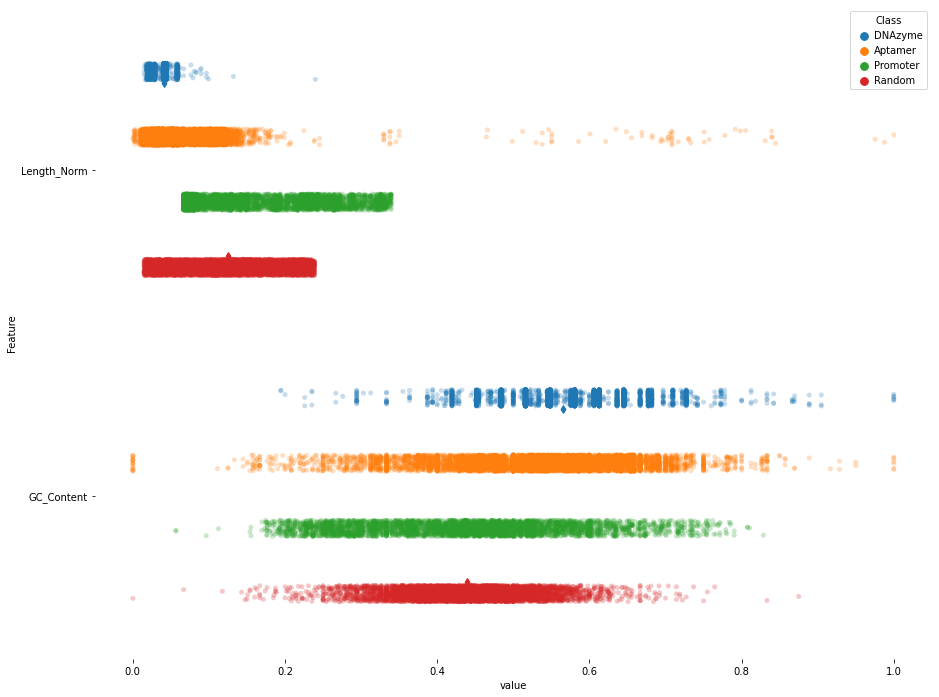
\includegraphics[width=0.9\linewidth]{./sequence_features.png}}
\end{figure}
Also the DNAzyme sequences were clustered, with sets from the same experiment designed to target the same gene.
This artificially increased the similarity of the DNAzymes and put heavy importance on specific k-mers that were important for that experiment by not for general DNAzyme-ness.
This bias is compounded by how short the sequences were and the very few sources of DNAzymes creating a highly over-fit model due to the artificial similarity of all the DNAzyme sequences.
At this point it appeared pointless to actually tune the hyperparameters due to how poor the DNAzyme data and due to time/data constraints I abandoned any further development of the model and used what I had.


\section*{Empirical Validation}
Ideally this project would provide a computational alternative to how DNAzymes might normally be optimized involving techniques like SELEX.
SELEX functions very well but it can be laborious and expensive and difficult to decide on some model parameters before starting.
Using a computational method will save significant amounts of time and resources, as well as allowing researchers to more easily experiment with simulation parameters.
So if a researcher can approximate a SELEX result with a simulated result that would be very beneficial and open up the use of DNAzymes (or potentially DNA Aptamers) for more research applications.

In order to do this I want to compare the output of SELEXzyme to that of a set of DNAzymes evolved \textit{in vitro} as done by \citet{valid}.
They did not preform SELEX but they did preform an assay testing the cleavage efficiency of thier DNAzymes to select the most effective ones.
So if my program works well it should ideally
\begin{itemize}
    \item output some DNAzymes similar to the best ones \citeauthor{valid} identified
    \item score the fitness of the \citeauthor{valid} DNAzymes similarly to their assay results
\end{itemize}

So the fitness rankings of the Abdelgany DNAzymes should be similar based on their assay results and my fitness function.
It is also possible that my program outputs no DNAzymes similar to the Abdelgany ones but still effective DNAzymes

The DNAzymes were taken from Table 1 from \citep{valid} (note, they show the targeted RNA sequence so I take the complement DNA for fitness evaluation).
The sequence for their DNAzyme target, AchR $\alpha$-subunit, was obtained from NCBI Gene.
%\link{here}{https://www.ncbi.nlm.nih.gov/CCDS/CcdsBrowse.cgi?REQUEST=CCDS&GO=MainBrowse&DATA=CCDS2261.1}.

The authors do not provide comprehensive fitness data, the most reliable fitness information they provided was that the DNAzymes followed a clear hierarchy of cleavage efficiency depending on the cleavage site (e.g. GT for 463GT(10+10)) which is $GT\leq A GC >>> AC$.

We can rank the DNAzymes by fitness determined by my program and see if they follow this pattern.

Using my model and the target gene cRNA my program calculated the following fitness values
\begin{center}
    \begin{tabular}{l|l}
    DNAzyme & Fitness \\
    \hline
    463GT(10+10) & 0.2\\
    463GT(13+9) & 0.2\\
    463GT(9+13) & 0.2\\
    472AT(10+10) & 0.18095238095238098\\
    472AT(13+9) & 0.1826086956521739\\
    472AT(9+13) & 0.1826086956521739\\
    476AC(10+10) & 0.19047619047619047\\
    685AC(13+9) & 0.16521739130434784\\
    694GT(13+9) & 0.2\\
    696AT(13+9) & 0.2\\
    765GT(13+9) & 0.2\\
    765GT(9+13) & 0.2\\
    799AC(13+9) & 0.18517395695217392\\
    801GT(13+9) & 0.1826086956521739\\
    801GT(9+13) & 0.1826086956521739\\
    805AT(13+9) & 0.1826086956521739\\
    808GC(13+9) & 0.1826086956521739\\
    811GT(10+10) & 0.18095238095238098\\
    811GT(13+9) & 0.1826086956521739\\
    811GT(9+13) & 0.1826086956521739\\
    811GT(13+13) & 0.1851851851851852\\
    \end{tabular}
\end{center}

So based on these fitness values they do seem to conform to our hierarchy with the exceptions of 696AT(13+9), 476AC(10+10), 799AC(13+9) which are considered more fit than they should be.
Based on how overfit the DNAzyme model was this was somewhat surprising but is still not a particularly impressive result.

The program was run with all default parameters except ``-lower 15'' and the fitness summary is shown here
\begin{center}
    \begin{tabular}{l|l}
        Fitness Stat & Value \\
        \hline
        Min             &0.15789473684210528\\
        25\% Quartile   &0.4789473684210526\\
        Mean            &0.4690277651388846\\
        75\% Quartile   &0.4789473684210526\\
        Max             &0.4789473684210526\\
        Std Dev         &0.04608867794884832\\
        CoV             &0.09826428491968045\\
    \end{tabular}
\end{center}
Qualitatively my DNAzymes are generally about half the length of the Abdelgany DNAzymes and contain much fewer C's, so they do appear to be fairly distinct.
Since these researchers have \textit{in vivo} validation for their DNAzymes it appears that my model is not particularly effective, especially since it is biasing to make sequences as short as possible due to how the DNAzyme model was trained.
However after increasing the lower bound from 10 to 15 results in a DNAzyme pool that look more similar to the Abdelgany DNAzymes and with a similar fitness distribution.
There is also larger redundancy in the final output as many of the sequences (the most fit) are identical and have identical fitness values.
\par
Ultimately this could be improved considerably by training a better DNAzyme model by finding a more representative data set.
Further one could incorporate biophysical knowledge into the fitness function to evaluate how the DNAzyme will fold and how that is conducive to cleavage.
DNAzymes are highly sensitive to environmental parameters like temperature an ion concentration so incorporating these into the model may also be effective without needing more training data.
\printbibliography
\end{document}


